\section{Numerical validation and statistical interpretation}
\label{sec:numerical}

Proofs of the results in this section appear in
Appendix~\ref{sec:proof-numerical}.


\subsection{Validation of the effective dynamics}
\label{subsec:numerics}

In this subsection, we specialize to logistic loss
and a quadratic penalty,
\[
    \ell(y,r)=\log(1+e^{-yr}),
    \qquad
    j(u)=\frac{u^2}{2},
\]
with symmetric confidence thresholds $\kappa_-=-\kappa_+<0$.
We compare trajectories generated by
Algorithm~\ref{alg:self-training} with particle simulations of
the effective recursion in
Definition~\ref{def:mean-field-recursion}.
Implementation details are available in the accompanying code
repository\footnotemark. 
Figure~\ref{fig:mean-field-validation} compares the resulting
macroscopic observables over repeated simulations.

\footnotetext{\url{https://github.com/ThierryRioual/HighDimensionalDynamicsOfSelfTraining}}

\begin{figure}[htbp] 
    \centering
    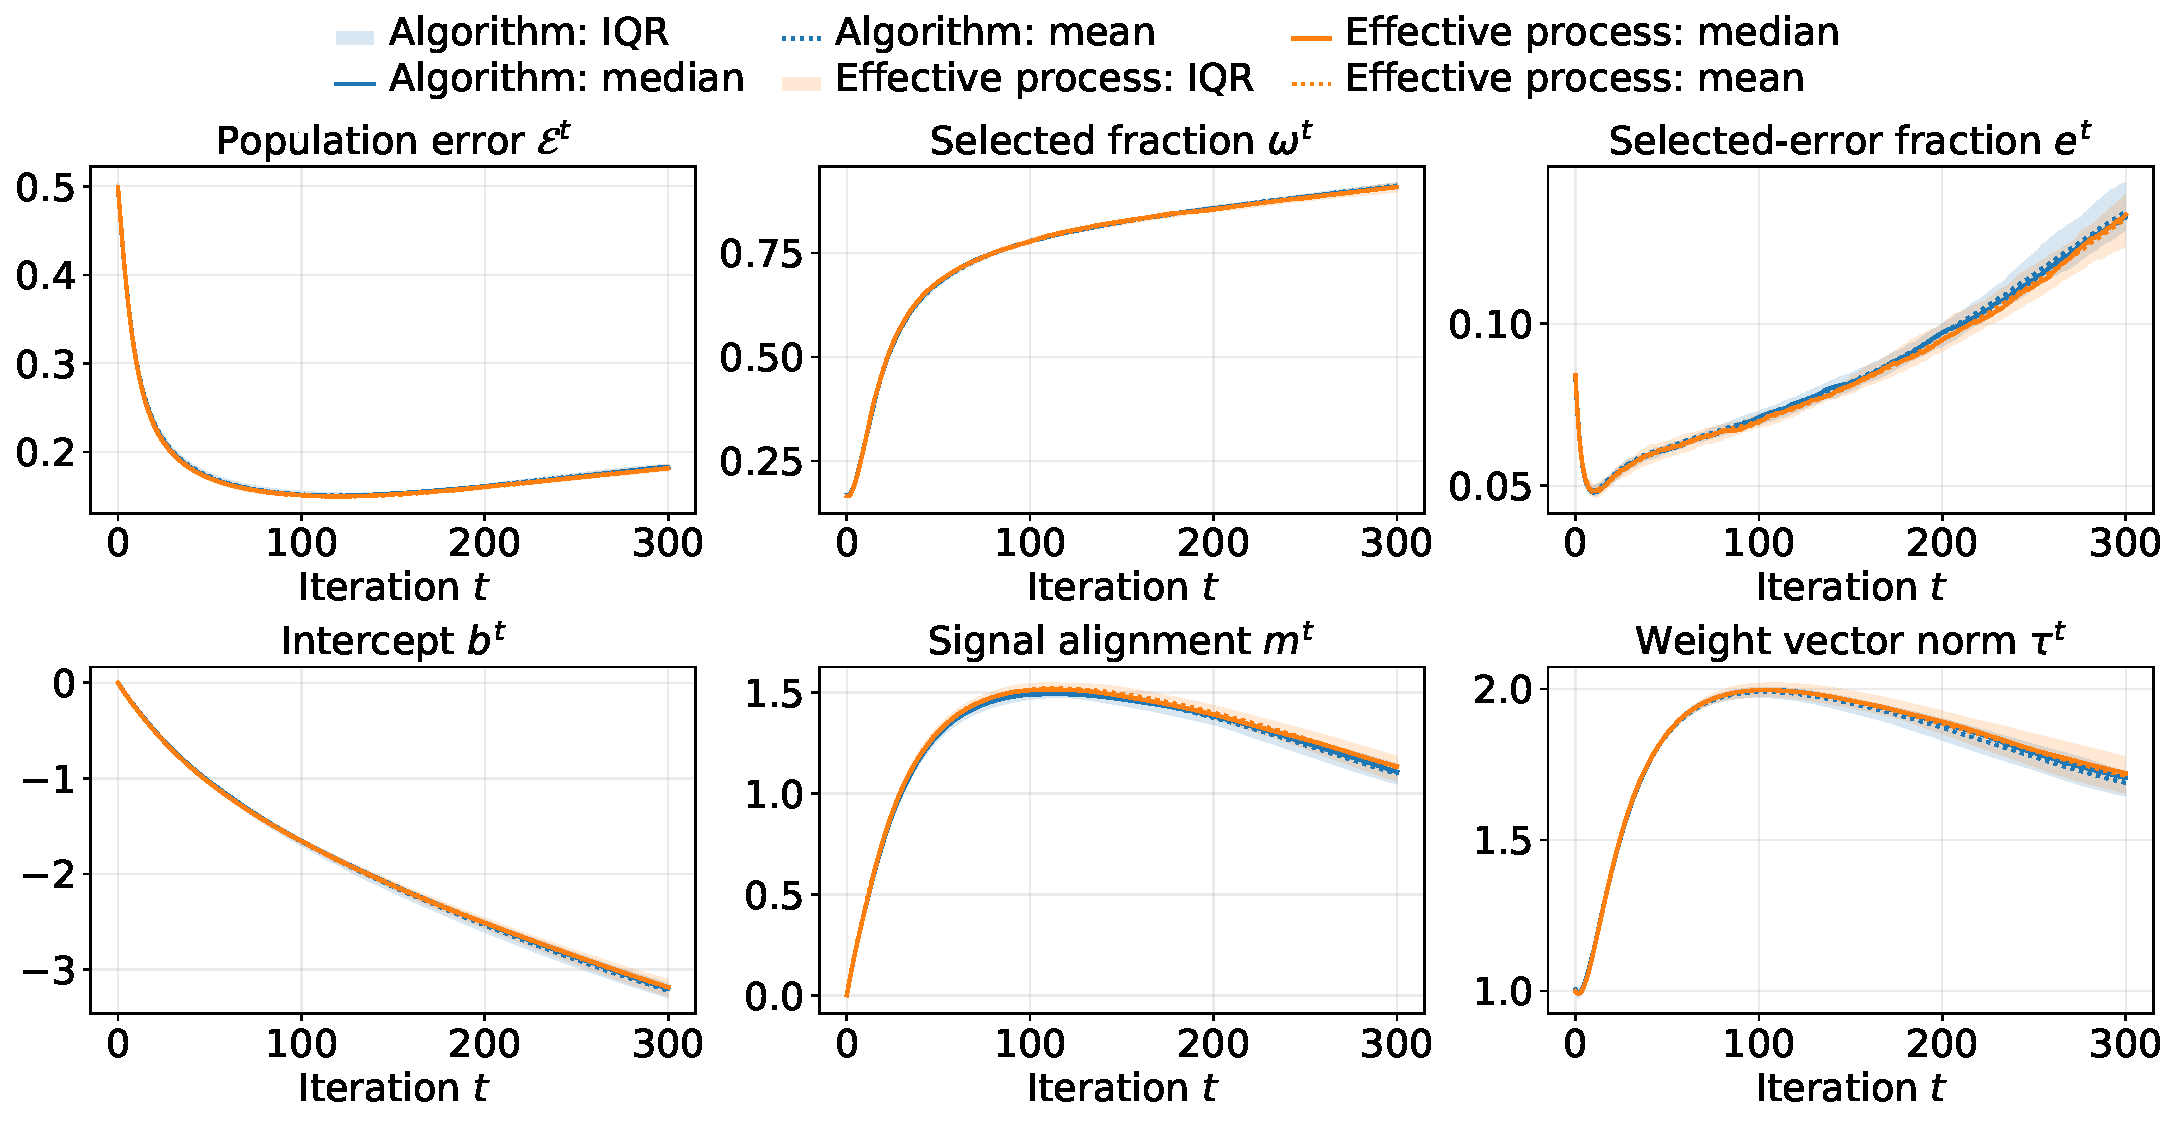
\includegraphics[width=1.0\textwidth]{figures/approximation_accuracy.pdf}
    
\caption{
Comparison of the self-training algorithm (blue) with the
particle approximation of the effective process (orange) over $20$ runs,
with $T=300$ iterations and seeds $42$--$61$.
Solid curves are medians, dotted curves are means, and shaded
regions are interquartile ranges.
The parameters are $d=2{,}000$, $\delta=8$, $\sigma=1$, $p=0.2$,
$\rho=0.1$, $\eta=0.1$, $\pi=5$, $\lambda=0.1$,  $\kappa_\pm=\pm\log4$, $b^{\mathrm{init}}=0$, with independent $w^{\mathrm{init}},\mu\sim\mathcal N(0_d,I_d)$.
Labels and supervision indicators are sampled independently
across observations with probabilities $p$ and $\rho$, respectively,
and held fixed throughout training.
Population errors use the configured class probability $p$.
The parameter-side and sample-side
effective processes are each simulated using $10{,}000$ particles.
}
    \label{fig:mean-field-validation} 
\end{figure}
The numerical experiments show that the effective predictions
closely track the finite-dimensional observables over the
displayed iteration horizon.
For the parameter setting and dimensions considered, this
agreement supports using the effective recursion to study
the statistical behavior of the algorithm.

\subsection{Classification error decomposition}
\label{subsec:classification-error}

By Corollary~\ref{cor:mean-field-observables}, the limiting
classification error depends on the normalized alignment
and intercept,
\[
    \bar\alpha^t
    :=
    \frac{\bar m^t}{\sigma\bar\tau^t},
    \qquad
    \bar\beta^t
    :=
    \frac{\bar b^t}{\sigma\bar\tau^t}.
\]
These are well defined at every finite time since
$\bar\tau^t>0$ by Lemma~\ref{lemma:mf-proof-nondegeneracy}.
We denote their finite-dimensional counterparts by
$\alpha^t$ and $\beta^t$, defined analogously when $\tau^t>0$.
The scalar alignment variables $\alpha^t,\bar\alpha^t$
should not be confused with the projection-coefficient
vectors $\alpha_t^{[w]},\alpha_t^{[g]}$ and their
barred counterparts.
Equation~\eqref{eq:mean-field-classification-error}
then becomes
\begin{equation}
    \bar{\mathcal E}^t
    =
    \mathcal E_{\bar p}(\bar\alpha^t,\bar\beta^t),
    \qquad
    \mathcal E_p(\alpha,\beta)
    :=
    p\,\Phi(-\alpha-\beta)
    +(1-p)\,\Phi(\beta-\alpha).
    \label{eq:normalized-classification-error}
\end{equation}
We use the Bayes classification error as a benchmark to evaluate the performance of the self-training algorithm.
Recall $\bar s_\mu=(\tilde{\mathbb E}[\tilde\mu^2])^{1/2}$
from \eqref{eq:s-mu-k-bar}, and write
$s_\mu:=\|\mu\|/\sqrt d$.

\begin{proposition}[Bayes classification error]
\label{prop:bayes-risk}
For every $\alpha>0$ and $p\in(0,1)$, the unique minimizer of
$\beta\mapsto\mathcal E_p(\alpha,\beta)$ is
\begin{equation}
    \beta_\star(\alpha;p)
    :=
    \frac{1}{2\alpha}\log\frac{p}{1-p}.
    \label{eq:classification-optimal-normalized-intercept}
\end{equation}
Suppose
Assumption~\ref{assumption:asymptotic-regime}
and Assumption~\ref{assumption:quenched-initialization} hold,
with $\bar s_\mu>0$.
For all sufficiently large $d$, the Bayes classification
error of the test mixture is
\[
    \mathcal E_{\mathrm B}
    :=
    \mathcal E_p\left(
        \frac{s_\mu}{\sigma},
        \beta_\star\left(\frac{s_\mu}{\sigma};p\right)
    \right).
\]
As $d\to\infty$, it converges to
\begin{equation}
    \bar{\mathcal E}_{\mathrm B}
    :=
    \mathcal E_{\bar p}(\alpha^\star,\beta^\star),
    \qquad
    \alpha^\star
    :=
    \frac{\bar s_\mu}{\sigma},
    \qquad
    \beta^\star
    :=
    \beta_\star(\alpha^\star;\bar p).
    \label{eq:bayes-classification-error}
\end{equation}
\end{proposition}
Next, we decompose the excess error
relative to the Bayes benchmark into alignment and intercept
regrets.
Define the smallest classification error attainable at a fixed
normalized alignment by
\[
    \mathcal E_p^{\mathrm{opt}}(\alpha)
    :=
    \inf_{\beta\in\mathbb R}
        \mathcal E_p(\alpha,\beta).
\]
For $\alpha>0$, Proposition~\ref{prop:bayes-risk} gives
\[
    \mathcal E_p^{\mathrm{opt}}(\alpha)
    =
    \mathcal E_p\bigl(\alpha,\beta_\star(\alpha;p)\bigr).
\]
For $\alpha\leq0$, the infimum equals $\min\{p,1-p\}$,
approached by predicting a single class.
Assuming $\bar s_\mu>0$, define the intercept regret and
alignment regret by
\begin{align}
    \bar{\mathcal R}_{\mathrm{int}}^t
    :=
    \mathcal E_{\bar p}(\bar\alpha^t,\bar\beta^t)
    -
    \mathcal E_{\bar p}^{\mathrm{opt}}(\bar\alpha^t),
    \qquad
    \bar{\mathcal R}_{\mathrm{align}}^t
    :=
    \mathcal E_{\bar p}^{\mathrm{opt}}(\bar\alpha^t)
    -
    \bar{\mathcal E}_{\mathrm B}.
    \label{eq:classification-regret-decomposition}
\end{align}
The intercept regret is nonnegative by definition.
Moreover, Cauchy--Schwarz gives
$|\bar\alpha^t|\leq\bar s_\mu/\sigma=\alpha^\star$.
For each fixed $\beta$,
\[
    \frac{\partial}{\partial\alpha}
        \mathcal E_p(\alpha,\beta)
    =
    -p\,\phi(\alpha+\beta)
    -(1-p)\,\phi(\beta-\alpha)
    <0,
\]
where $\phi=\Phi'$.
Thus $\mathcal E_p^{\mathrm{opt}}$ is nonincreasing, and
the alignment regret is also nonnegative.
Their sum gives the excess classification error:
\[
    \bar{\mathcal E}^t-\bar{\mathcal E}_{\mathrm B}
    =
    \bar{\mathcal R}_{\mathrm{int}}^t
    +
    \bar{\mathcal R}_{\mathrm{align}}^t.
\]
The intercept regret measures the gap between the current error
and the infimum attainable by varying the intercept while
holding the weights fixed.
The alignment regret is the remaining excess error after this
optimization.

For finite-dimensional trajectories with $\tau^t>0$,
$s_\mu>0$, and $p\in(0,1)$, the conditional test error satisfies
\[
    \mathcal E^t=\mathcal E_p(\alpha^t,\beta^t),
    \qquad
    |\alpha^t|\leq\frac{s_\mu}{\sigma}.
\]
The first identity follows from the Gaussian test-score law
used in the proof of
Corollary~\ref{cor:mean-field-observables};
the second follows from Cauchy--Schwarz.
Consequently, the same decomposition applies with
$(p,\alpha^t,\beta^t)$ and the finite-dimensional Bayes error
$\mathcal E_{\mathrm B}$ defined in
Proposition~\ref{prop:bayes-risk}, with both regret terms nonnegative.
Figure~\ref{fig:class-imbalance-regret} compares the error
trajectories and their regret decompositions in balanced and
imbalanced settings.
\begin{figure}[htbp] 
    \centering
    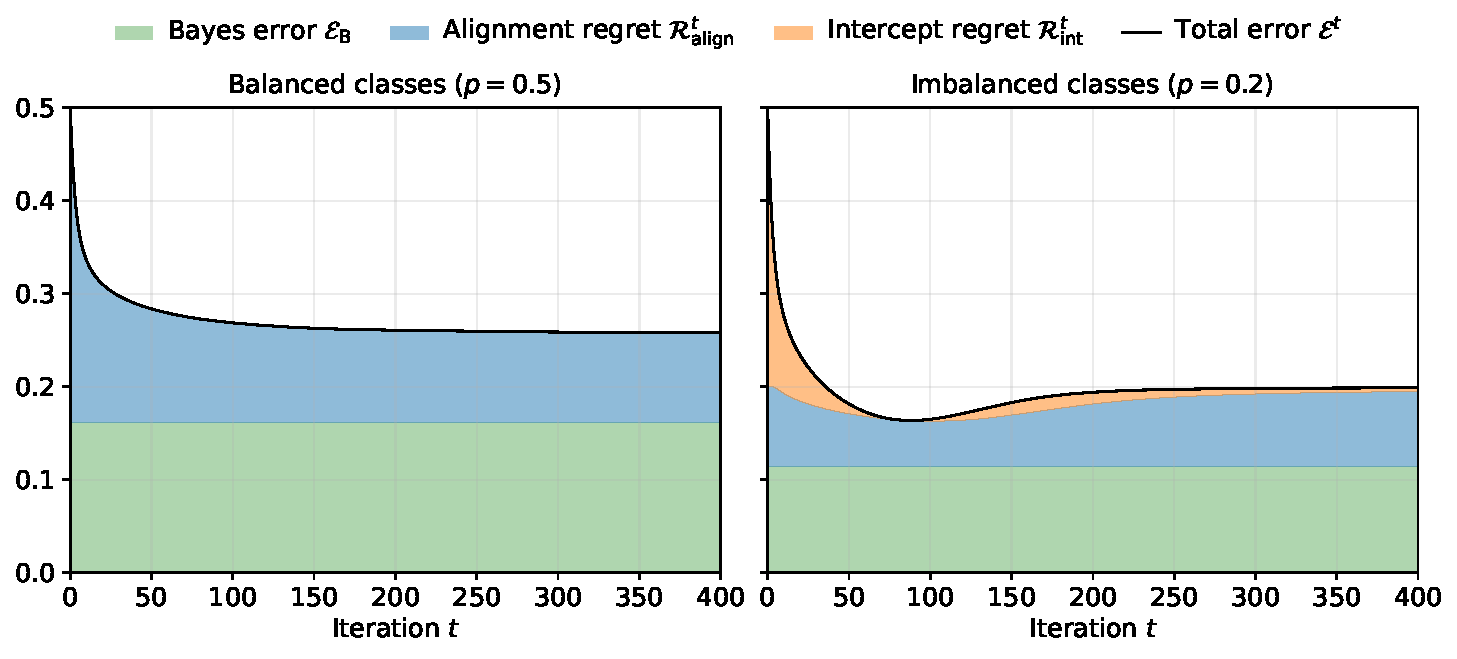
\includegraphics[width=\textwidth]{figures/statistical_behavior_comparison.pdf}
\caption{
Classification-error decomposition for balanced ($p=0.5$, left)
and imbalanced ($p=0.2$, right) classes, using one realization
of the self-training algorithm in each case, with $T=400$
iterations and seed $49$.
The stacked layers represent Bayes error, alignment regret,
and intercept regret; each layer's thickness gives its
contribution to the total error (black).
Both experiments use logistic loss, the quadratic penalty, $d=5{,}000$, $\delta=8$, $\sigma=1$,
$\rho=0.05$, $\eta=0.2$, $\pi=2$, $\lambda=0.1$, $\kappa_\pm=\pm\log4$, $b^{\mathrm{init}}=0$, with independent $w^{\mathrm{init}},\mu\sim\mathcal N(0_d,I_d)$.
Labels and supervision indicators are sampled independently
across observations with probabilities $p$ and $\rho$, respectively,
and held fixed throughout training.
Population errors use the configured class probability $p$.
}
\label{fig:class-imbalance-regret} 
\end{figure}

\subsection{Intercept dynamics and class imbalance}
\label{subsec:intercept-dynamics}

Our experiments show that the classification performance of
self-training depends strongly on the hyperparameters and
the data distribution, consistent with previous empirical
evaluations of self-training and semi-supervised learning
\cite{oliver2018realistic,su2021realistic}.

In balanced settings, our experiments show that classification error decreases consistently throughout training.
In imbalanced experiments, however, we repeatedly observe an
initial decrease followed by an increase, producing a U-shaped
error curve over the training iterations.
Figure~\ref{fig:class-imbalance-regret} illustrates these
contrasting trajectories.
Similar risk trajectories arise in the self-training regression
model of Wu et al.~\cite{wu2026selftraininghelpshurtsdenoising}.
In our imbalanced experiments, intercept regret begins
increasing before alignment regret.
We also observe that the normalized intercept moves beyond
its classification-optimal value as training progresses.
Figure~\ref{fig:mean-field-validation}, which uses a related
imbalanced configuration, shows the evolution of the
intercept, signal alignment, and weight norm.
Meanwhile, classification error approaches the majority-class
benchmark, equal to $0.2$ in the right panel of
Figure~\ref{fig:class-imbalance-regret}.
Together, these observations suggest an important role for
intercept feedback in the deterioration observed under
class imbalance.

The importance of intercept dynamics is also emphasized by
Takahashi~\cite{takahashi2026role}, who studies self-training
on imbalanced Gaussian mixtures using fresh unlabeled batches
and stagewise minimization, and proposes fixing the intercept
as a heuristic.
Takanami et al.~\cite{takanami2025effect} also study intercept
drift and bias fixing under imbalance in a repeated-data
self-distillation setting. 
These considerations motivate a closer examination of the
intercept and weight updates.
The following proposition distinguishes the contributions
of pseudo-label imbalance and pseudo-label correctness.

\begin{proposition}[Weighted pseudo-label contributions]
\label{prop:weighted-pseudo-label-contributions}
Suppose the hypotheses of Theorem~\ref{theorem:trajectory} hold
and, in addition,
\[
    -y\ell'(y,r)\geq0,
    \qquad
    y\in\{-1,+1\},\quad r\in\mathbb R.
\]
For every finite $t\geq0$, define
\[
    \tilde A^t
    :=
    -\tilde{\mathfrak c}^{\,t}
        \ell'(\tilde{\mathfrak c}^{\,t},\tilde r^t)
    \geq0,
\]
using the convention $\ell'(0,r)=0$.
Then the following identities hold.
Their algebra does not require the sign condition;
that condition ensures $\tilde A^t\geq0$ and supports
the subsequent interpretation.

\begin{enumerate}[label=(\roman*),wide]
    \item \emph{Weighted pseudo-label contributions.}
    The unlabeled residual satisfies
    \begin{align}
        \tilde{\mathbb E}[\tilde g_{\mathcal U}^t]
        &=
        \tilde{\mathbb E}\left[
            \tilde A^t
            \left(
                \mathbf1_{\{\tilde{\mathfrak c}^{\,t}=-1\}}
                -
                \mathbf1_{\{\tilde{\mathfrak c}^{\,t}=+1\}}
            \right)
            \,\middle|\,\tilde\Delta=0
        \right],
        \label{eq:weighted-pseudo-label-imbalance}
        \\
        \tilde{\mathbb E}
            [\tilde Y\tilde g_{\mathcal U}^t]
        &=
        \tilde{\mathbb E}\left[
            \tilde A^t
            \left(
                \mathbf1_{\{\tilde{\mathfrak c}^{\,t}=-\tilde Y\}}
                -
                \mathbf1_{\{\tilde{\mathfrak c}^{\,t}=\tilde Y\}}
            \right)
            \,\middle|\,\tilde\Delta=0
        \right].
        \label{eq:weighted-pseudo-label-correctness}
    \end{align}
    For logistic loss,
    \[
        \tilde A^t
        =
        \frac{|\tilde{\mathfrak c}^{\,t}|}
             {1+e^{|\tilde r^t|}}.
    \]

    \item \emph{Intercept and overlap updates.}
    Writing
    \[
        \bar\zeta^t
        =
        \tilde{\mathbb E}[\tilde g_{\mathcal L}^t]
        +
        \pi\tilde{\mathbb E}[\tilde g_{\mathcal U}^t],
        \qquad
        \bar\chi^t
        =
        \tilde{\mathbb E}[\tilde Y\tilde g_{\mathcal L}^t]
        +
        \pi\tilde{\mathbb E}[\tilde Y\tilde g_{\mathcal U}^t],
    \]
    Definition~\ref{def:mean-field-recursion} gives
    \begin{equation}
        \bar b^{t+1}-\bar b^t
        =
        -\eta\bar\zeta^t
        \label{eq:statistical-intercept-drift}
    \end{equation}
    and
    \begin{equation}
        \bar m^{t+1}-\bar m^t
        =
        -\eta\left[
            \bar\chi^t\bar s_\mu^2
            +
            \lambda
            \tilde{\mathbb E}
                [\tilde\mu\,j'(\tilde w^t)]
            +
            \sigma
            \sum_{s=0}^{t}
                \bar\gamma^{[g]}(t,s)\bar m^s
        \right].
        \label{eq:statistical-overlap-update}
    \end{equation}
\end{enumerate}
\end{proposition}

Equation~\eqref{eq:weighted-pseudo-label-imbalance}
measures the derivative-weighted imbalance between negative
and positive selected pseudo-labels.
Its contribution to the intercept increment is
$-\eta\pi\tilde{\mathbb E}[\tilde g_{\mathcal U}^t]$.
Thus, when $\pi>0$, a larger weighted mass of negative
pseudo-labels pushes the intercept downward, whereas a larger
weighted mass of positive pseudo-labels pushes it upward.
Equation~\eqref{eq:weighted-pseudo-label-correctness}
instead compares incorrect and correct selected pseudo-labels.
Through the explicit signal term
$-\eta\pi\tilde{\mathbb E}
[\tilde Y\tilde g_{\mathcal U}^t]\tilde\mu$,
correct pseudo-labels contribute toward the signal and
incorrect pseudo-labels contribute in the opposite direction.
The complete overlap update
\eqref{eq:statistical-overlap-update} also contains the labeled
contribution, regularization, and memory.
For a quadratic penalty, $j(u)=u^2/2$, its regularization
expectation reduces to $\bar m^t$.
These identities distinguish the quantities driving the updates,
but explaining intercept overshoot requires understanding
how the weighted pseudo-label imbalance evolves jointly
with the weights.
This raises the question:

\medskip
\emph{Under what conditions does self-training drive the
normalized intercept beyond its classification-optimal value,
and how does this interact with signal alignment and
classification error?}
\medskip

The effective recursion characterizes the transient dynamics,
but extracting an analytical explanation of intercept
amplification remains challenging.
Its coefficients depend self-consistently on the trajectory
laws, while nonlinear feedback and memory prevent a closed
description in terms of the intercept and alignment alone.
Long-time convergence and equilibrium behavior of effective
processes have been studied in
\cite{celentano2026highdimensionalasymptoticsordermethods,
fan2025dynamicalmeanfieldanalysisadaptivereplica,
chen2025learningsingleindexmodel};
Theorem~\ref{thm:effective-process-convergence} also establishes
convergence for the present recursion.
These convergence results do not by themselves provide
quantitative conditions for intercept amplification.
We leave such a characterization under class imbalance
as an open problem.

Nevertheless, an exact reference case arises when the classes
are balanced within both supervision populations, the thresholds
are symmetric, and the initial effective intercept is zero.
Under a corresponding symmetry of the loss, the labeled and
unlabeled contributions to the intercept update each vanish
at every iteration.

\begin{proposition}[Preservation of a zero intercept under symmetry]
\label{prop:zero-intercept-symmetry}
Suppose the hypotheses of Theorem~\ref{theorem:trajectory}
hold. Assume that the loss satisfies
\begin{equation}
    \ell'(-y,-r)=-\ell'(y,r),
    \quad y\in\{-1,+1\},\quad r\in\mathbb R,
    \label{eq:loss-label-score-symmetry}
\end{equation}
and that the classes are balanced within each supervision
population:
\begin{equation}
    \tilde{\mathbb P}(\tilde Y=+1\mid\tilde\Delta=a)
    =\frac12,
    \qquad a\in\{0,1\}.
    \label{eq:balance-within-supervision}
\end{equation}
If $\kappa_-=-\kappa_+$ and $\bar b^0=0$,
then, for every $t\geq0$,
\begin{equation}
    \bar b^t=0,
    \qquad
    \tilde{\mathbb E}[\tilde g_{\mathcal L}^t]
    =
    \tilde{\mathbb E}[\tilde g_{\mathcal U}^t]
    =0.
    \label{eq:zero-intercept-all-times}
\end{equation}
Moreover, for every finite horizon $T$,
\begin{equation}
    (\tilde Y,\tilde\Delta,\tilde r^0,\ldots,\tilde r^T)
    \overset{\mathrm d}{=}
    (-\tilde Y,\tilde\Delta,-\tilde r^0,\ldots,-\tilde r^T).
    \label{eq:joint-score-reflection}
\end{equation}
\end{proposition}

Every differentiable margin loss
$\ell(y,r)=\varphi(yr)$ satisfies
\eqref{eq:loss-label-score-symmetry}, since
$\ell'(y,r)=y\varphi'(yr)$; this includes logistic loss.
Under the hypotheses of
Proposition~\ref{prop:zero-intercept-symmetry},
$\bar p=1/2$ and $\bar\beta^t=0$, so
\begin{equation}
    \bar{\mathcal E}^t=\Phi(-\bar\alpha^t).
    \label{eq:symmetric-classification-error}
\end{equation}
Classification performance is therefore determined entirely
by normalized alignment. At times when $\bar\alpha^t\geq0$,
the intercept regret vanishes. Any deterioration in the
effective classification error must be accompanied by a
decrease in $\bar\alpha^t$.
For the finite-dimensional iterates,
Theorem~\ref{theorem:trajectory} also gives
\[
    \max_{0\leq t\leq T}|b^t|
    \xrightarrow{\mathbb P}0
\]
for every fixed finite horizon $T$.
Thus exact preservation of the effective intercept corresponds
to an asymptotically vanishing finite-dimensional intercept
on fixed horizons.
